\documentclass{article}
\usepackage[utf8]{inputenc}
\usepackage[margin=1in]{geometry}
\usepackage{graphicx}
\usepackage{natbib}
\usepackage{enumitem}
\usepackage{array}
\usepackage{gensymb}
\usepackage{indentfirst}
\graphicspath{ {Images/} }
\usepackage{float}
\usepackage[table,xcdraw]{xcolor}
\usepackage{amsmath}

\title{Physics 111A Fall 2016- Lab 9\\
Lab View Programming}
\author{Joshua Levy\\Lab Partner: Alex Chuang}
\date{November 6th, 2016}

\begin{document}

\maketitle

\section{Lab Write Up}
%1
\subsection{Discerning signals in the presence of noise}
    For this section of the lab, we utilized the program "Noisy Signal Generator.vi", and made the following observations:
    \begin{itemize}
        \item With noise set to 0, we saw that the signal looked like a pure sine wave.
        \item With averaging off and with large noise, it was hard to discern what the sine wave's frequency response was because the amplitude of the noise obscured the amplitude of the sine wave in the frequency response domain.
        \item With averaging on, the fourier (fast fourier transformed) amplitude of the RMS noise was reduced and this amplitude only increased as we increased the noise level.
        \item With a noise level of 40 and averaging on, we began to decrease the averaging depth to see what was the lowest averaging depth to be able to still spot out the original sine signal. We saw the signal with an averaging depth as low as two with the continuous regeneration of noise and averaging options turned on.
        \item As we increased the noise level, we needed to increase the averaging dept in order to spot out the original signal.
        \item With a noise level of 100, we could spot the original signal at an averaging depth of 8.
    \end{itemize}
    
%2
\subsection{}
    We loaded the program "Visual Noise.vi". We followed the directions on the lab handout and were able to spot out the following pictures at the following noise levels (pictures below are numbered):
    \begin{enumerate}
        \item Noticed Abraham Lincoln at a noise level of 70.
        \item Noticed image of person from many years ago (this person was less recognizable to me because I was not exposed to him) at a noise level of 30.
        \item Noticed Marilyn Monroe at a noise level of 50.
        \item Noticed Martin Luther King at a noise level of 40.
        \item Noticed Mona Lisa at a noise level of 140.
        \item Noticed Statue of Liberty at a noise level of 100.
        \item Noticed John F. Kennedy at a noise level of 110.
        \item Noticed Einstein's iconic image at a noise level of 170.
    \end{enumerate}
    Picture's 1, 2, and 3 were grayscale noise. The colored noise made it harder for me to make out the images. Overall, it was easiest to make out the signal/image through high levels of noise when I was standing back and the continuous regeneration option was turned on. That setup was like averaging the signal and having greater averaging depth, as in the first section. We can see that these higher scores  (able to see the image at higher noise settings) arose during images 7 and 8, when I used the aforementioned settings.
    
%3
\subsection{}
    See signature page
    
%4
\subsection{}
    \begin{figure}[H]
        \centering
        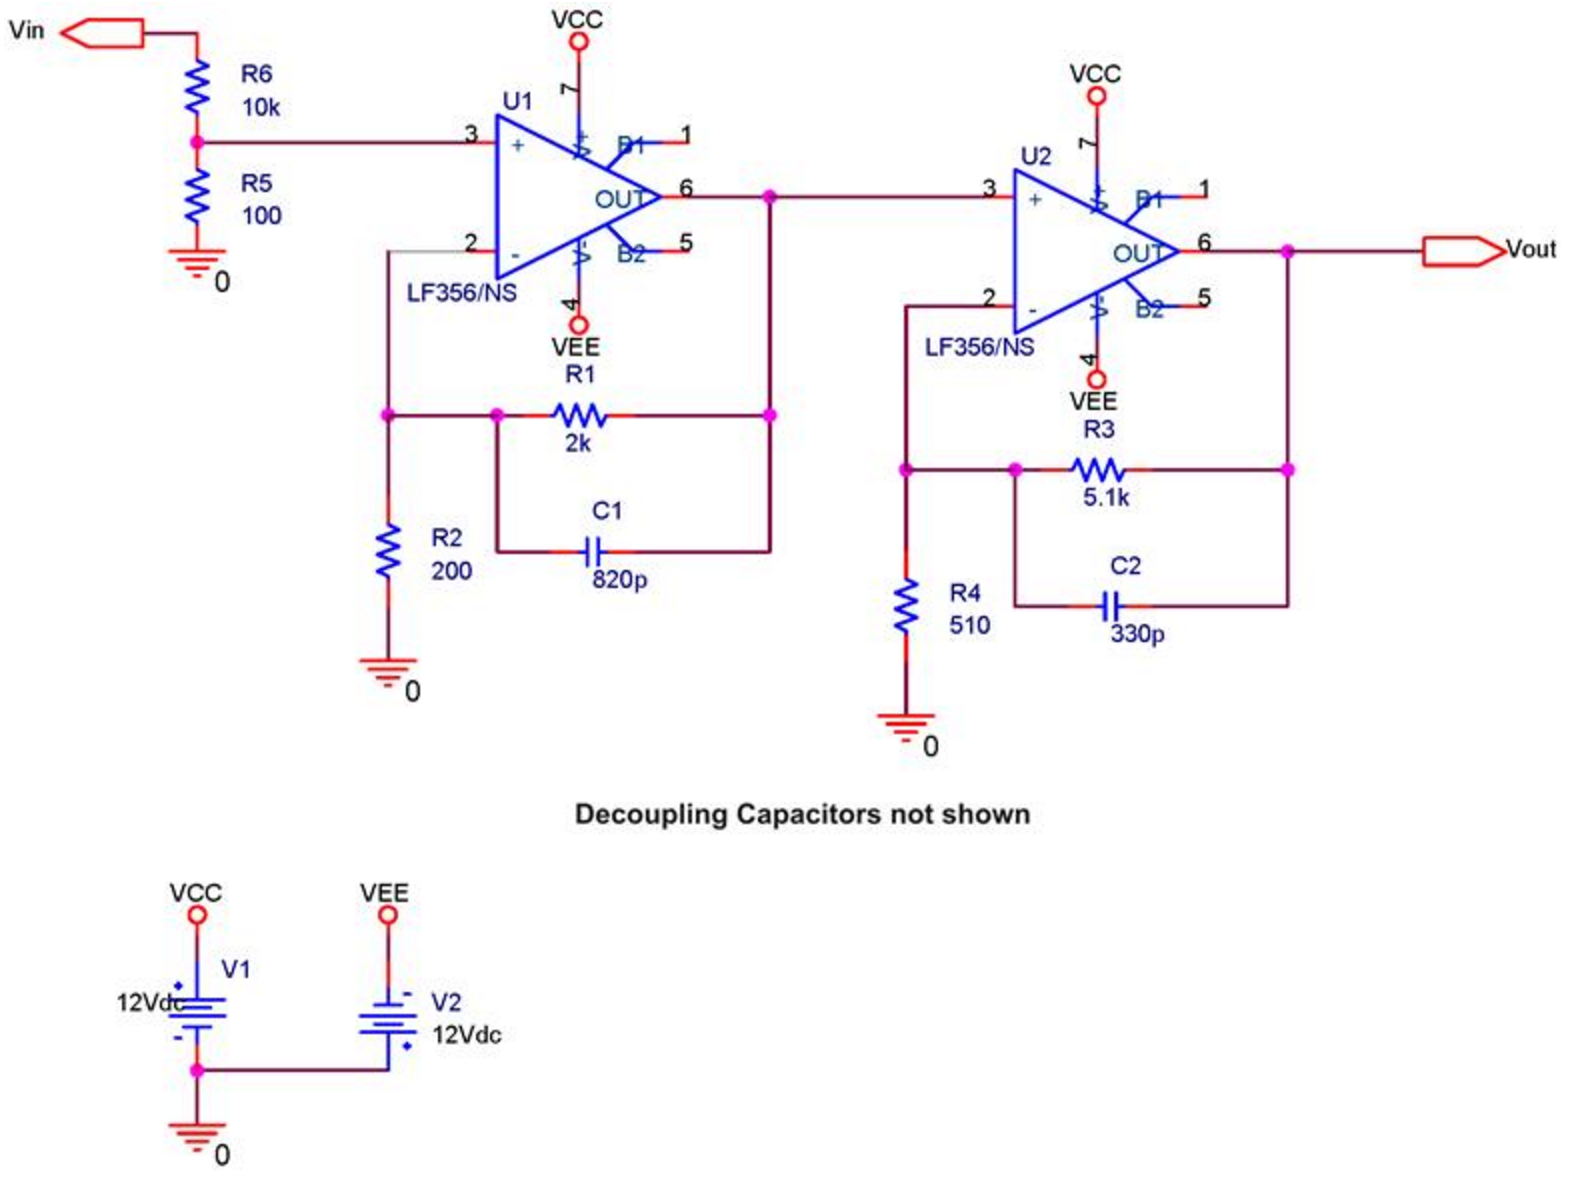
\includegraphics[scale = 0.5]{4.png}
        \caption{Amplifier Circuit with Voltage Divider \cite{lab9}}
        \label{fig:my_label}
    \end{figure}
    We debugged the above circuit with a 1kHz, 0.1V signal connected to the voltage divider. In the prelab, we predicted the gain of the circuit to be:
    \begin{equation}
        G = \frac{V_{out}}{V_{in}} = \frac{R_5}{R_6 + R_5}*(\frac{R_1}{R_2}+1)*(\frac{R_3}{R_4}+1)
    \end{equation}
    and plugging in the following resistor values:
    \begin{table}[H]
        \centering
        \caption{Resistors and Capacitors Measured for the Above Circuit}
        \label{my-label}
        \begin{tabular}{ll}
        \textbf{Circuit Components} &  \\ \cline{1-1}
        \textbf{$R_1$} & 2.01k \\
        \textbf{$R_2$} & 198.8$\Omega$ \\
        \textbf{$R_3$} & 4.99k \\
        \textbf{$R_4$} & 501.6$\Omega$ \\
        \textbf{$R_5$} & 103.3$\Omega$ \\
        \textbf{$R_6$} & 10.08k \\
        \textbf{$C_1$} & 822pF \\
        \textbf{$C_2$} & 328.2pF
        \end{tabular}
        \end{table}
    We expected to find a gain of:
    \begin{equation}
        G \approx 1.234
    \end{equation}
    Inputting our wave of 1$V_{pp}$, we attained a $V_{in}$ of 96 mV and $V_{out}$ of 124 mV, corresponding to a gain of 1.29, with some error. So we see that our circuit is behaving as expected and is debugged.
    
%5
\subsection{}
    \begin{figure}[H]
        \centering
        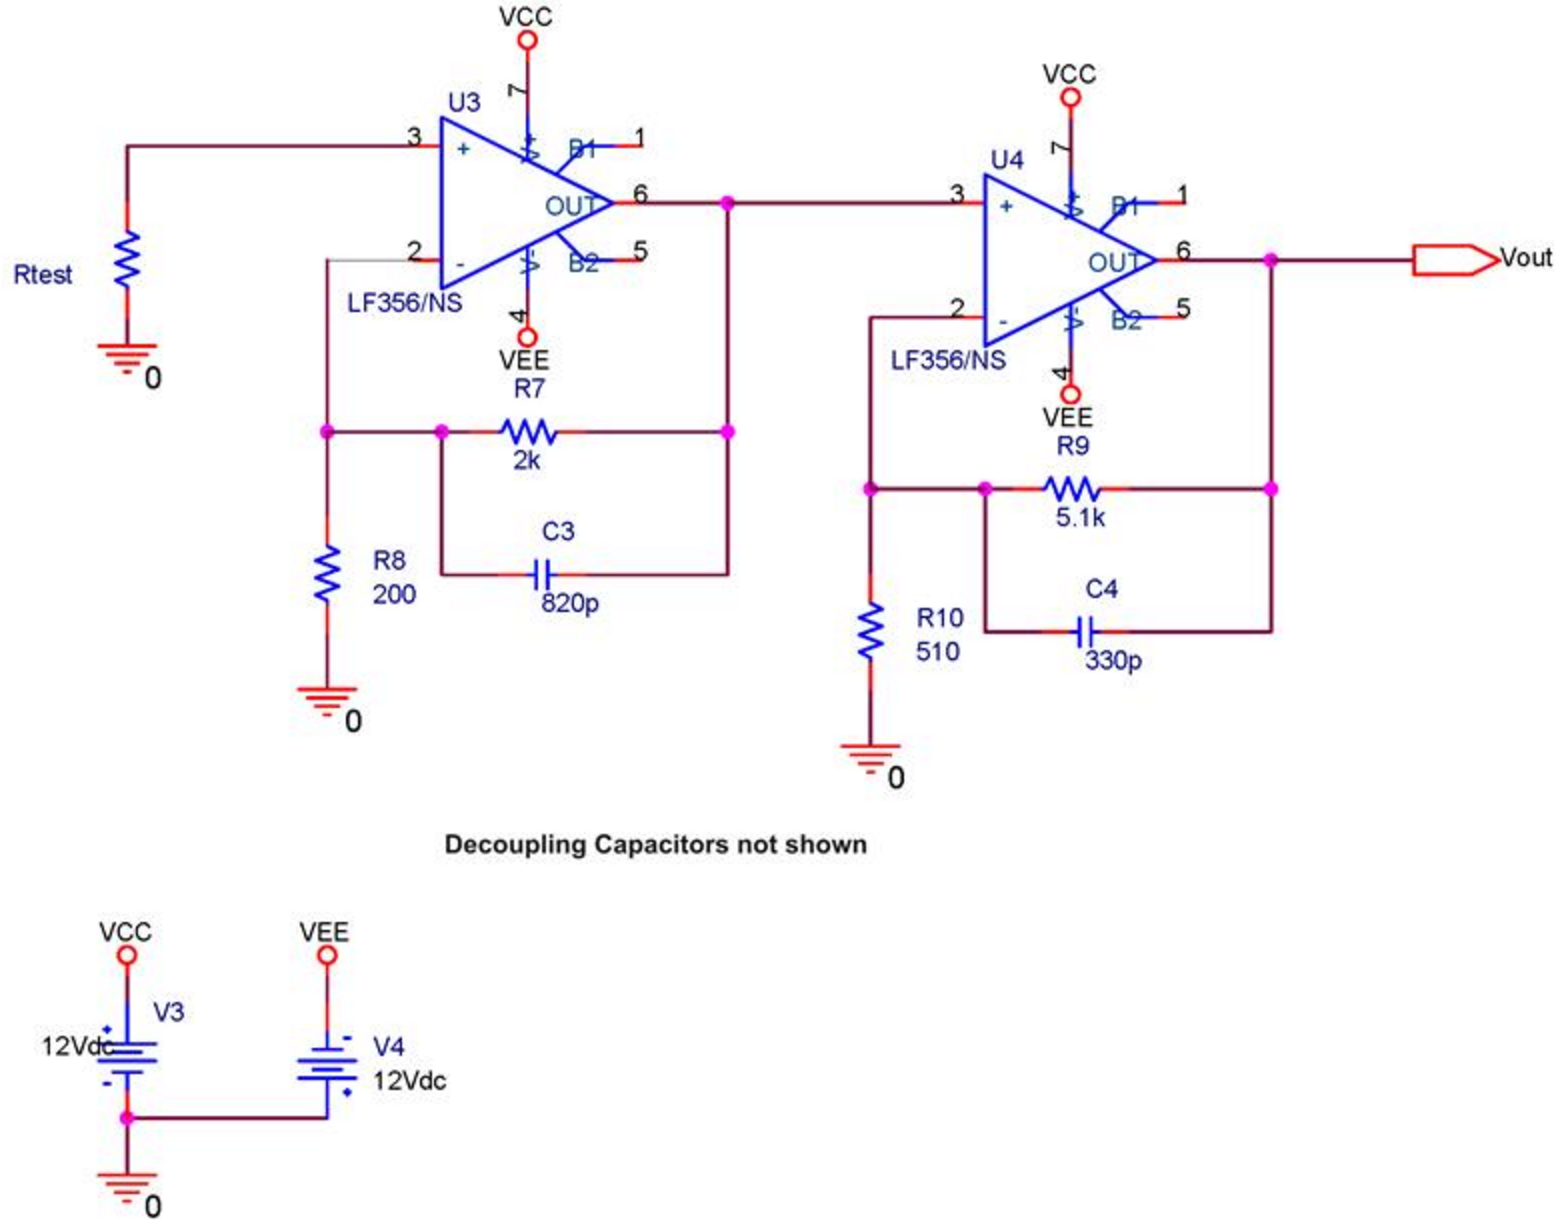
\includegraphics[scale = 0.5]{5.png}
        \caption{Amplifier Circuit Setup Used to Calculate $k_B$ Boltzmann Constant \cite{lab9}}
        \label{fig:my_label}
    \end{figure}
    We ran the circuit from the previous section and found our transfer function to be:
    \begin{figure}[H]
        \centering
        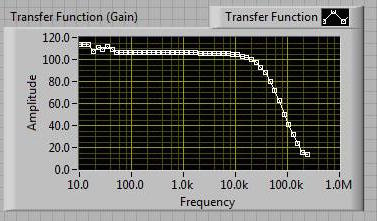
\includegraphics[scale = 0.8]{5b.jpeg}
        \caption{Transfer Function of Amplifier Circuit with Voltage Divider \cite{lab9}}
        \label{fig:my_label}
    \end{figure}
    We see that the amplitude is flat in the region between frequencies 60Hz and about 10kHz, and the flat region corresponds to a gain of 106 from the voltage divider onwards. We removed the voltage divider and connected a 100k resistor (measured to be 100.1k).
    
%6
\subsection{}
    See signature page
    
%7
\subsection{}
    My partner and I constructed a labview program that would take Johnson noise of various resistors and use it to measure the Boltzmann constant. We programmed into our labview program the function \cite{lab9}:
    \begin{equation}
        k_B = \frac{N}{4TRFG^2}(V_{meas}^2 - V_{intr}^2)
    \end{equation}
    where R is the resistor used, $V_{meas}^2$ is the $V_{RMS}^2$ for our circuit with a resistor, and $V_{intr}^2$ is the squared intrinsic RMS voltage noise level of the amplifier measured with R = 0 ($V_{instr}$ measured to be 4.1138 * $10^{-5}$V), F is the frequency range, which we plugging in 500kHz, T was the room temperature ($\approx 293K$), and N was the number of samples read, which was 1000. G was the gain listed in section [1.5], which was 106. Plugging in the resistor values below and the values described above, we measured the following Boltzmann constant values and compared them to the expected Boltzmann constant $k_B = 1.38064852 * 10^{-23} J/K$:
    \begin{table}[H]
        \centering
        \caption{Boltzmann Constant Measured Using Johnson Noise Formula for Amplifier Circuit with Various Resistors}
        \label{my-label}
        \begin{tabular}{llll}
        \textbf{R ($\Omega$)} & \textbf{$V_{RMS}$(V)} & \textbf{$k_B$ ($10^{-23}$*J/K)} & \textbf{Absolute Error ($10^{-23}$*J/K)} \\ \hline
        10.03k & 0.00005965 & 2.82938 & 1.44938 \\
        100.1k & 0.00011 & 1.56 & 0.18 \\
        1M & 0.00045 & 3.0498 & 1.6698
        \end{tabular}
        \end{table}
    We see from the absolute error that the boltzmann constants found are on the same order of magnitude as the expected value.
    





\section{Signature Page}
\begin{figure}[H]
    \centering
    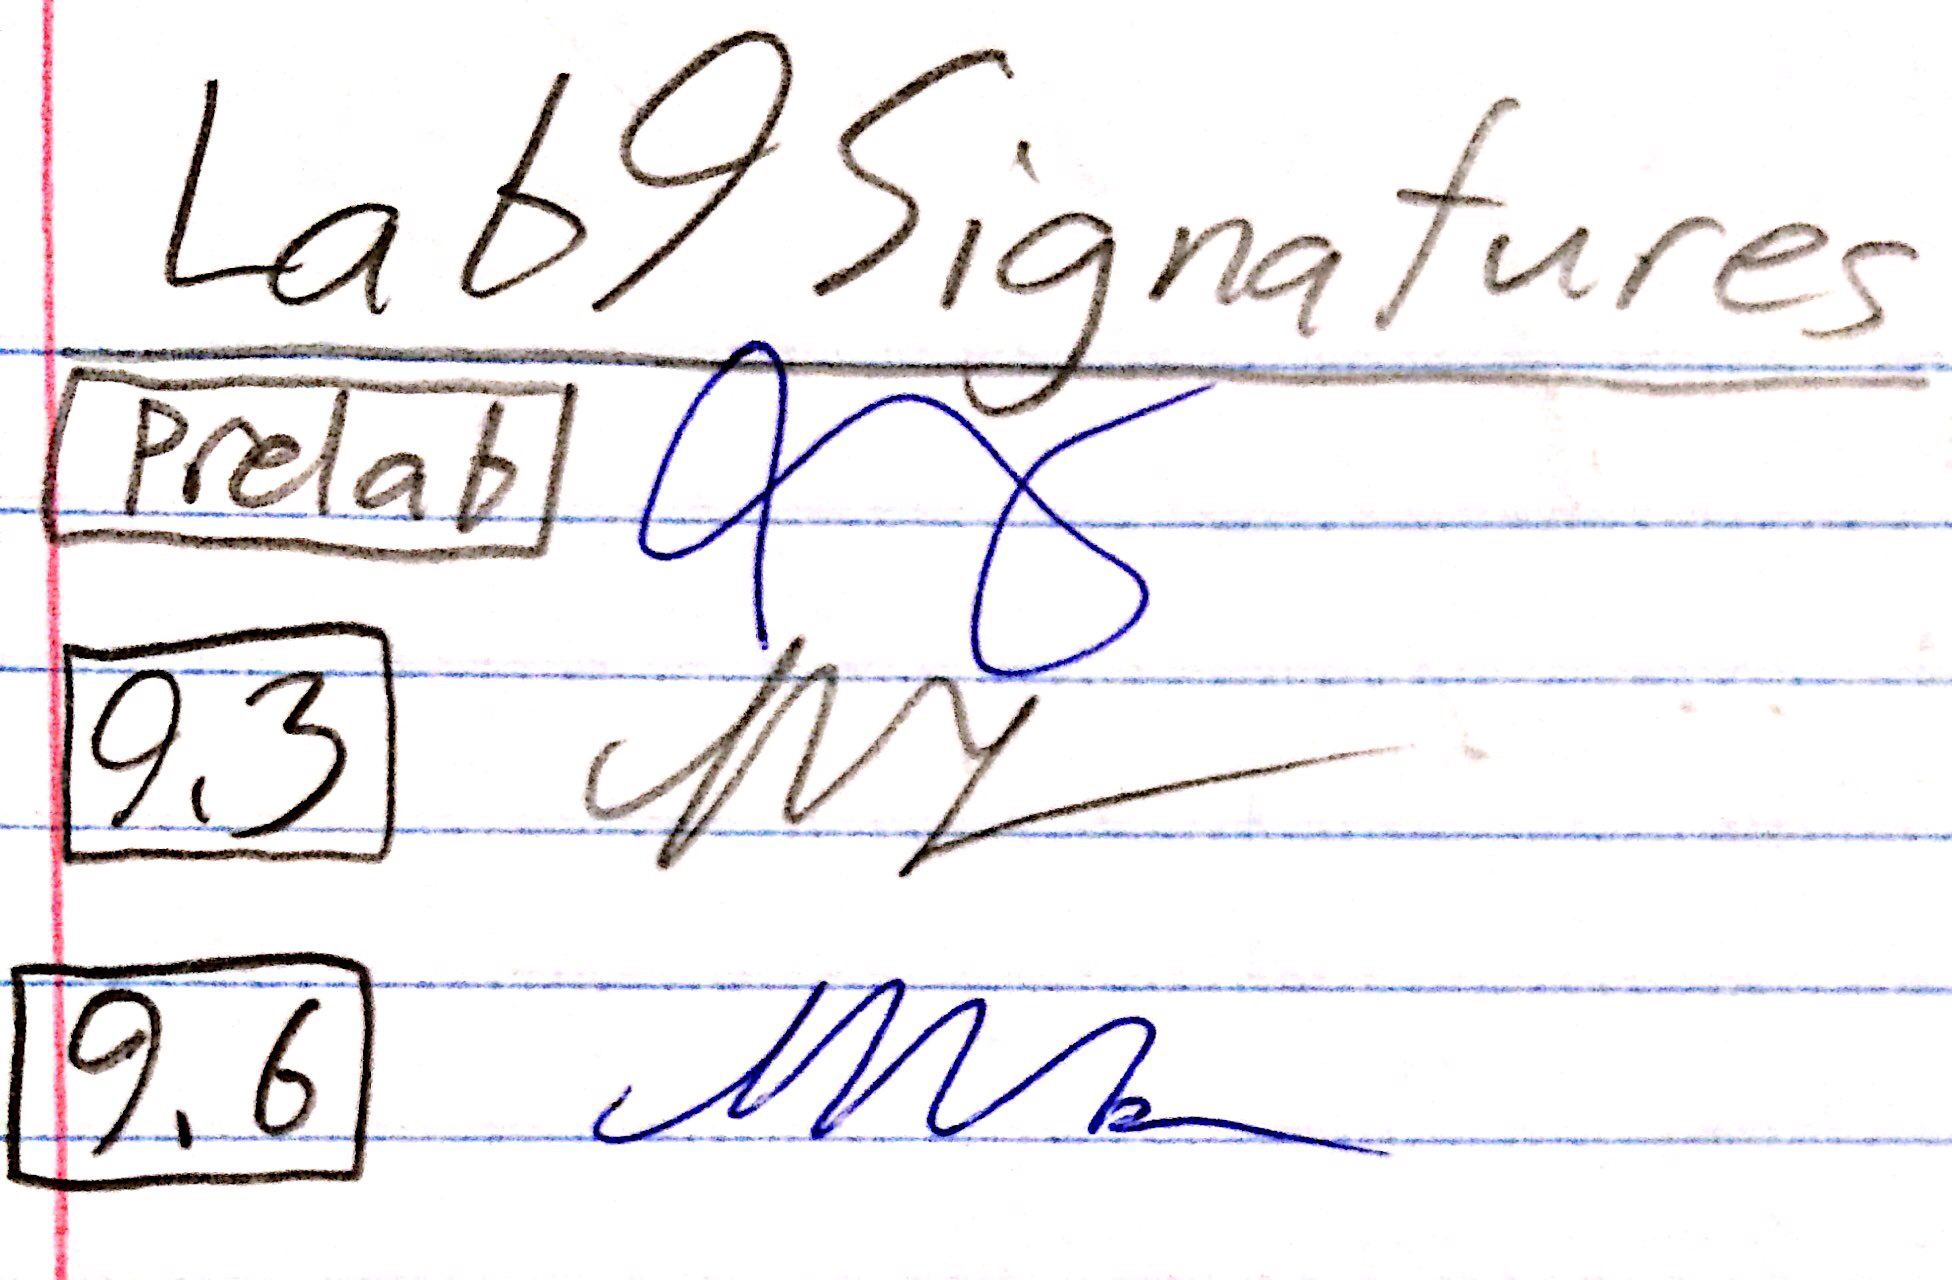
\includegraphics[scale = 0.15]{sig.JPG}
    \caption{Signatures}
    \label{fig:my_label}
\end{figure}



\bibliography{joshbib}{}
\bibliographystyle{plain}


\end{document}

\begin{figure}[H]
    \centering
    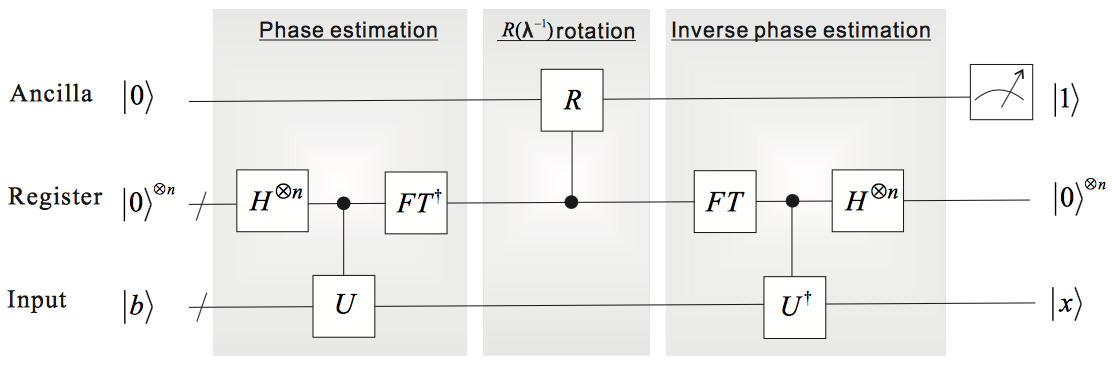
\includegraphics[scale = 0.5]{1.png}
    \caption{Caption}
    \label{fig:my_label}
\end{figure}

